In this chapter, we propose the first approach to long tail advertising in sponsored search. We propose that advertisers should bid upon high level concepts instead of keywords in ad space auctions. We formulate the problem as an optimization objective to maximize the revenue of the search engine and give an approximate algorithm for it along with an end-to-end framework. 




\section{Motivation and Basic Idea}
Search queries follow a long tail distribution with a small head of frequent queries and a long tail of infrequent queries. Advertising on tail queries is hard mainly due to the data sparsity problem as the frequency of tail queries is very less. Also, it has been observed that advertisers tend to bid for head keywords in the ad space auctions because of the individually high reach of head keywords. Further, the long tail of search queries makes it quite difficult for the advertisers to identify all the relevant keywords for their products. The stated factors result in significant amount of under-utilization of ad space of the tail queries which is identified as the research gap.

In this chapter, we propose an approach to exploit the ad space of tail keywords. We propose that instead of bidding on keywords advertisers should bid upon high level concepts in ad space auctions. The motivation behind bidding on concepts is inspired from the fact that each concept can be logically composed of multiple keywords, head and tail alike. The reach of an individual tail query keyword may not be desirable. However, the reach of a set of keywords containing both head and tail query keywords or just tail keywords can be considered equivalent to head keywords. For example, the word ``airline" is very popular in the AOL search query logs but the words like \{ first, jack, pennsylvania, mount, wildlife \} are not as popular. A group of such keywords could be created to compete with the head keywords in ad space auctions. 

The key idea of this approach is to sell groups of keywords in ad space auctions. The keywords are grouped together through high level concepts. We propose that in ad space auctions of search keywords, advertisers should bid upon high level concepts instead of individual keywords. Bidding on higher level concepts is achieved through a two-level taxonomy. During ad space auctions, advertisers are shown the first level of the taxonomy and are asked to select a node which seems to be the most relevant to their product. For example, if an advertiser wants to bid upon shopping, he/she will select the concept \textit{Shopping} from the first level nodes. Thus, we propose to add a middle layer of concepts through a taxonomy during the bidding process such that an advertiser would choose a concept which would ultimately translate to a set of keywords, compared to the present approach where the advertiser is responsible for selecting all the desired keywords. Figure \ref{bidding_mechanism} (a) shows the keywords based approach where advertisers bid upon keywords where advertiser $A_1$ chose to bid upon keywords $K_1$ and $K_2$ and advertiser $A_2$ chose to bid upon keywords $K_2$ and $K_3$. Figure \ref{bidding_mechanism} (b) shows the concept-based bidding approach where advertisers bid on concepts through a taxonomy which are composed of search keywords.

\begin{figure}
  \centering
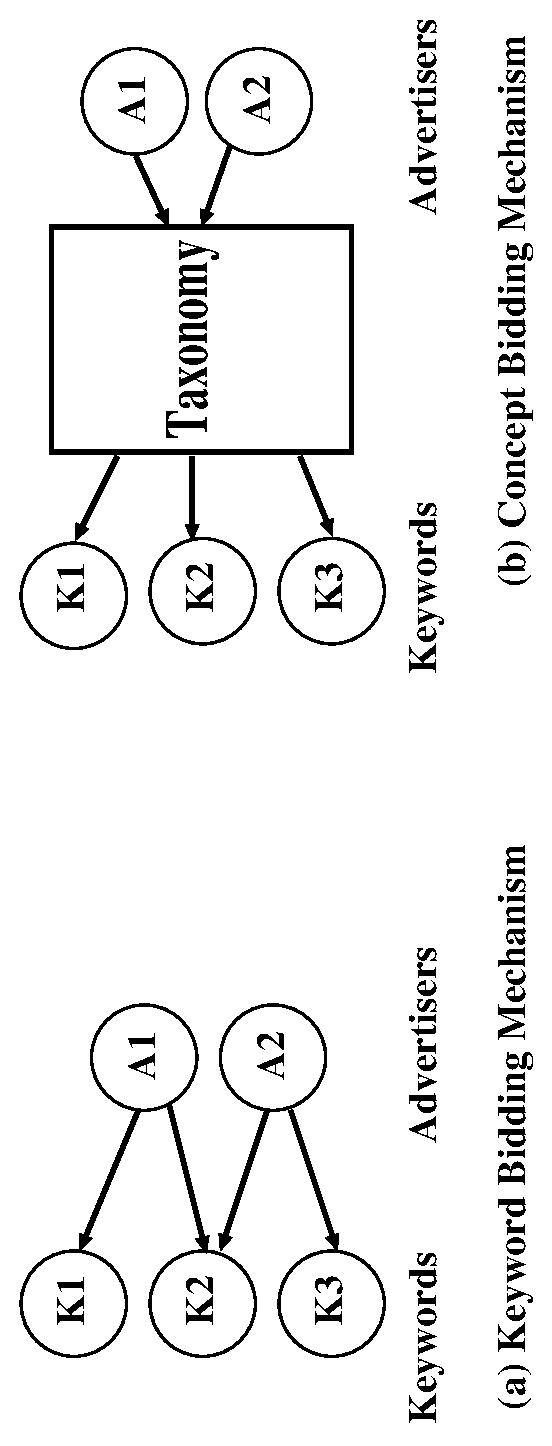
\includegraphics[scale=0.4,angle = 270]{visuals/bidding_old_new.eps}
  \caption{Sponsored search bidding: keywords based bidding and concept-based bidding}
  \label{bidding_mechanism}
\end{figure}


In the proposed approach, each advertiser selects a node to bid upon and groups of children nodes of bidding nodes are assigned to the advertisers. To form such groups of children nodes, we mine coverage patterns from session-based transactions derived from search query logs. Each search session is modelled as a transaction with queries occurring in the session as the items. Each query is further replaced by the corresponding first and second level nodes from the bidding taxonomy. Coverage patterns are extracted from these session based transactions using the approach proposed in \cite{srinivas2014mining}. Compared to the arbitrary grouping on nodes, the extracted coverage patterns would help in identifying sets of nodes of the children nodes which ensure maximal overlap, thereby reducing the repetition of ads in the same session. We propose to perform a matching between the extracted coverage patterns and the advertising demands. We propose to model the matching as an optimization objective to maximize the revenue of the search engine and propose an end-to-end framework to realize the matching and to allow the advertisers to bid on a two-level taxonomy.



The rest of the chapter is structured as follows. In Section \ref{Ch4ProposedModel}, the proposed model is discussed. The proposed framework in discussed in Section \ref{ch4Framework} including the optimization objectives and algorithms followed by experiments in Section \ref{ch4Experiments}, and assumptions and limitations in Section \ref{Ch4Discussion}. Section \ref{ch4Summary} summarizes the chapter.

 

\section{Proposed Model}


\label{Ch4ProposedModel}


When a query is fired by a user to the search engine, the query is first classified according to the taxonomy and the advertisers who have been assigned the corresponding nodes are the candidate advertisers for the query. Thus, in the proposed model, a middle layer of coverage patterns has been added between keywords and advertisers as shown in Figure \ref{fig:proposedModelJournal}. The left most side of the diagram shows one disjoint set as the advertisers and the right side has another disjoint set as queries with coverage patterns of taxonomy nodes in the middle. 
\begin{figure}
	\centering
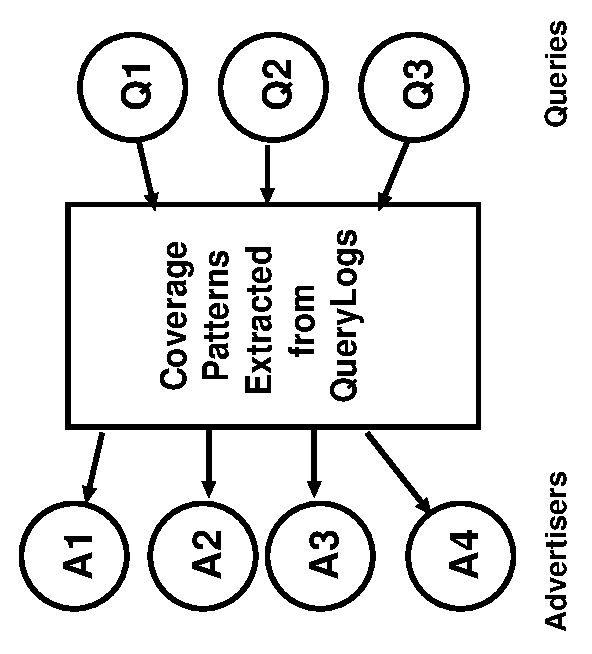
\includegraphics[scale=0.3,angle = 270]{visuals/proposedModelDSAA.eps}
	\caption{Proposed model }
	\label{fig:proposedModelJournal}
\end{figure}

Through the proposed model, it is possible to exploit more ad space of the tail queries as each advertiser is allocated a set of concepts and each concept would contain a mix of head and tail keywords. Thus, all the keywords, head or tail, would be considered for advertising based on their relevancy rather than frequency.

Using the proposed model, we have defined an end-to-end framework for allocating incoming queries to advertisers. The proposed framework is discussed in the next section.





\section{Proposed Framework}
\label{ch4Framework}

The proposed framework is shown in Figure \ref{fig:proposedArchitectureJournal}. It has the following steps.


\begin{figure}
	\centering
	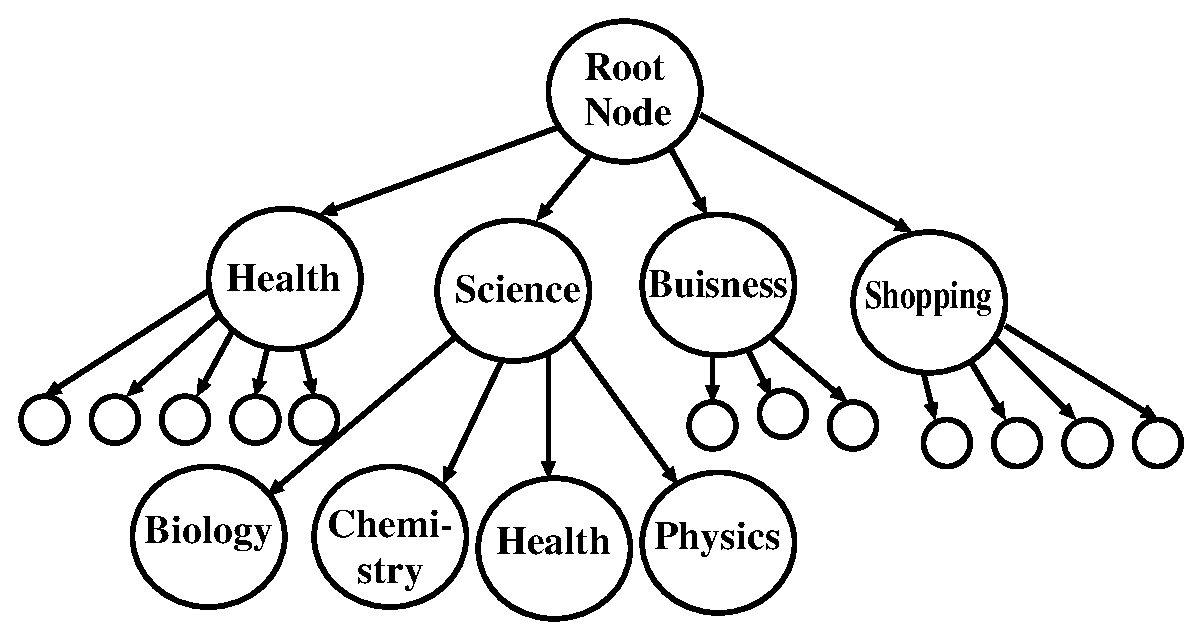
\includegraphics[scale=0.4]{visuals/our_taxonomy.eps}
	\caption{Example of a concept taxonomy}
	\label{taxonomy:example}
\end{figure}




\begin{enumerate}[label=(\roman*).]
\item \textbf{{\em Analysis of Query}}: This step is same as the original sponsored search systems approach with an addition to classify the incoming query using a taxonomy. We have proposed the approach by considering  a two-level taxonomy. A dummy root node is level zero, nodes at level one are termed as concepts and nodes at level two are sub-concepts of their parent concept as shown in Figure \ref{taxonomy:example}. Given a query, we extract the corresponding concept and sub-concept pair from the concept taxonomy along with other information as required by the sponsored search system. (Note that we propose that the advertiser should bid upon a node in the taxonomy. In this study, we investigate the setting such that advertisers are only bidding on the nodes in level 1. It is possible to extend the  proposed approach by considering a taxonomy of higher number of levels with appropriate modifications,  which will be explored in the next chapter.)

\item \textbf{{\em Retrieve Relevant Ads from the Matching}}: This step identifies the relevant advertisers for a given query. Compared to the proposed approach, we have modified it such that it takes search query and the matching between advertisers \& coverage patterns (which is the output of the allocation of concepts to advertisers component) as inputs. Using the matching, we retrieve advertisers who have been allotted the coverage pattern containing the sub-concept of the incoming query. In the next subsection, we will explain the component of allocation of concepts to advertisers and how the matching is computed.



\item \textbf{{\em Bidding}}: Ad space on each search query is sold by means of auctions. Each advertiser bids for the ad slots. This bid can be static or dynamic. (This step is the same as the standard sponsored search approach.) 


\item \textbf{{\em Ranking of  Advertisers}}: Based on the bid amount and other relevant parameters like CTR and ad-query relevance, advertisers are ranked to be shown on the query's results page. (This step is also same as the standard sponsored search approach.)


\begin{figure*}
	\centering
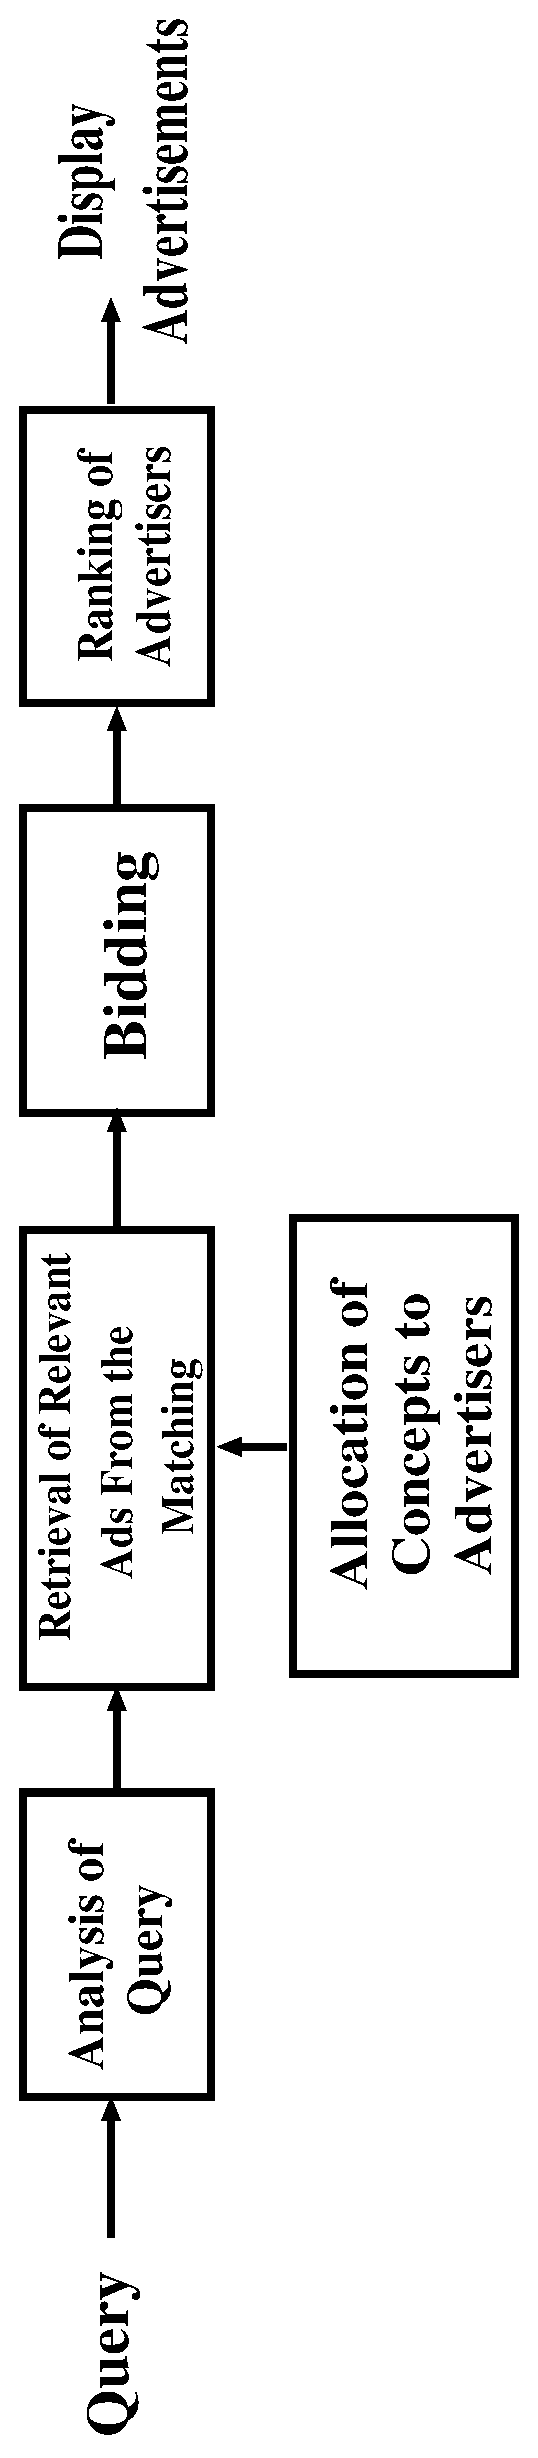
\includegraphics[scale=0.37,angle = 270]{visuals/ProposedArchitectureJournal.eps}
	\caption{Proposed Architecture}
	\label{fig:proposedArchitectureJournal}
\end{figure*}

\end{enumerate}

In the remaining section, we will discuss how to allocate concepts to advertisers and compute the matching between advertisers and coverage pattern.

\textbf{\subsection{Allocation of concepts to advertisers}}
In this sub-section, we explain the process of allocation of the concepts of taxonomy to advertisers. The process of allocation is divided into the following steps, as shown in Figure \ref{allocation}.

\begin{figure*}
	\centering
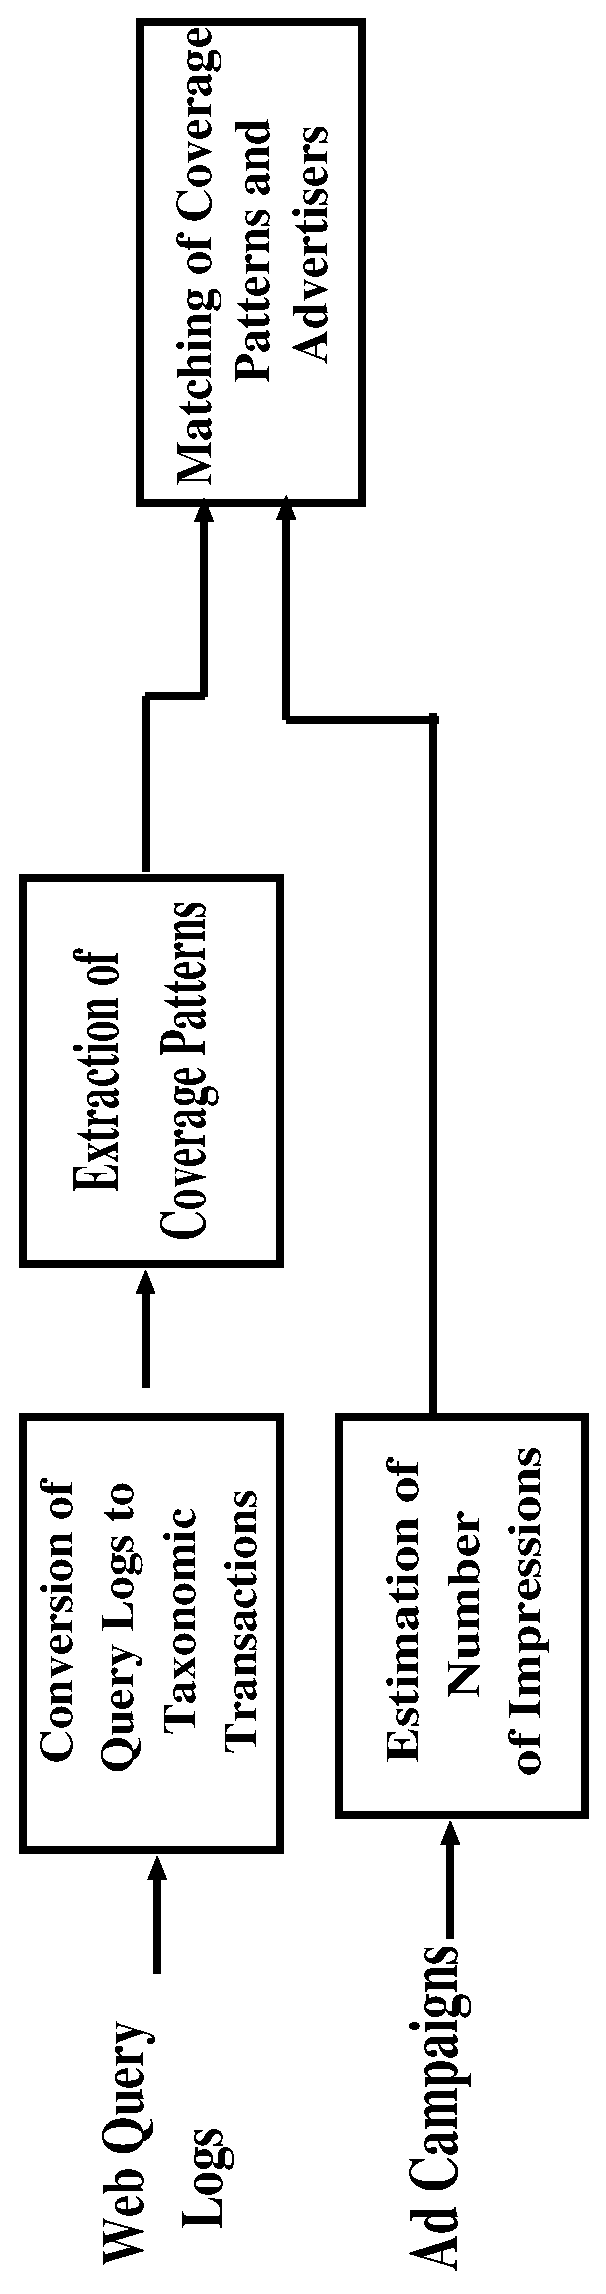
\includegraphics[scale=0.37,angle = 270]{visuals/allocation_dsaa.eps}
	\caption{Allocation of concepts to advertisers}
	\label{allocation}
\end{figure*}




\begin{enumerate}[label=(\roman*).]
\item {\em Conversion of Query Logs to Taxonomic Transactions}

\item {\em Extraction of Coverage Patterns}

\item {\em Estimation of Number of Impressions (of Advertisers)}

\item {\em Matching Coverage Patterns and Advertisers}
\par

\end{enumerate}


In the rest of the subsection, we explain each step in detail.



\textbf{\subsubsection{Conversion of Query Logs to Taxonomic Transactions}}


We extract search sessions from the given web query logs. The search sessions are transformed into session based transactions. Queries in the same session form the items of the corresponding session transaction. We further transform each transaction by replacing each query with it's concept and sub-concept pair using the taxonomy. The transformed transaction is termed as `taxonomic transaction'.


Example 2: We explain all the steps of the framework through a running example by considering a set of advertisers who chose to bid on the concept of {\it Science}. {\it Biology, Chemistry, Technology, Environment, Physics} and {\it Agriculture} are the sub-concepts of {\it Science}.  Conversion of  query logs into transactions is shown in Table \ref{table:queries} and Table \ref{table:transactions}. Table \ref{table:queries} shows the sessions extracted from the query logs. These queries are classified into concepts and sub-concepts according to the taxonomy. For example, in session with session--id 1, there are three queries of concept {\it Science} out of which one belongs to the sub-concept {\it Biology} and two belong to the sub-concept {\it Chemistry}. To create a transaction, we used the session--id, concept and the sub-concepts that occur in the session. For the first session, it will be 
$<1, Science, \{Biology, Chemistry\}>$. 
Similarly, the rest of the query logs are converted to taxonomic transactions to mine coverage patterns. \par

\begin{table}

\centering
\caption{Sample Sessions \label{table:queries}}
\begin{tabular}{|l|l|l|l|}
\hline
Session-id & Query & Concept & Sub-concept \\ \hline
1 & chromatography & Science & Biology \\
1 & o-toulene & Science & Chemistry \\
1 & dimethylene & Science & Chemistry \\
2 & wood boring bees & Science & Agriculture \\
2 & anthrenus carpet & Science & Biology \\
3 & artficail intelligence & Science & Technology \\
4 & tree symbolism & Science & Environment \\
5 & internship computer science & Science & Technology \\
5 & ipod prices & Science & Technology \\
6 & health plan & Science & Biology \\
\hline
\end{tabular}

\end{table}





\begin{table}

\centering
\caption{Taxonomic Transactions \label{table:transactions}}
\adjustbox{max width=\columnwidth}{
\begin{tabular}{|l|l|l|}
\hline
Sr. No & Concept & Sub-concepts \\ \hline
1 & Science & \{Biology, Chemistry\} \\
2 & Science & \{Agriculture, Biology\} \\
3 & Science & \{Technology\} \\
4 & Science & \{Enviornment\} \\
5 & Science & \{Technology\} \\
6 & Science & \{Biology\} \\
\hline
\end{tabular}}
\end{table}




\textbf{\subsubsection{Extraction of Coverage Patterns}}
Extraction of coverage patterns from the search query posed two main challenges which are stated as below.

\begin{enumerate}[label=(\Alph*)]

\item Coverage patterns are mined from the perspective of unique visitors considering each transaction as one visitor. However, in order to leverage coverage patterns in computational advertising, the knowledge of coverage patterns needs to be converted to either impressions or clicks. 

We propose to convert number of visitors of a coverage pattern into impressions. We will later use this knowledge of impressions to match coverage patterns to advertisers.

To estimate the number of impressions from the coverage patterns, we used set theory. From the definition of coverage patterns, a coverage set of a coverage pattern $X$ is the union of all the transactions of each item in $X$ and overlap ratio is the ratio of number of common transactions between the first $n-1$ items of coverage pattern $X$ and the last item, $n^{th}$ item to the number of transactions having the $n^{th}$ candidate item. Thus, OR is roughly half of the intersection ratio between $X$ and the candidate item. 

One key assumption that we have made in the estimation is that we don't take into account the frequency of each item in a transaction and consider it one, if present and zero otherwise. From overlap ratio and coverage support, the task was to find the number of times both items have occurred together in the transaction dataset. In set theory, the following theorem gives the total number of items having both $A$ and $B$.
\begin{equation}
 n(A) + n(B) = n(A \cup B) + n(A \cap B) 
\end{equation}

Our requirement is to estimate $n(A) + n(B)$ where coverage support would be $n(A \cup B)$ and $\frac{Overlap Ratio}{2}$ would be $n(A \cap B)$. Hence, number of impressions by a given coverage pattern, $X$ is computed as followed.

\begin{equation}
 Impressions(X) = (CS(X) + \frac{OR(X)}{2}) * |D| 
\end{equation}
where $|D|$ is the total number of transactions or this case, number of sessions.

\item In the proposed approach, we allocated coverage patterns of taxonomy nodes to the advertisers. Given a single advertiser, which coverage pattern to allocate is the challenge we faced. To resolve the issue of selection of coverage patterns, we propose to rank coverage patterns. A ranking amongst coverage patterns could be established by multiple methods including only overlap ratio (to reduce repetition), only coverage support (to get the most number of impressions) or a function of both overlap ratio and coverage. In this approach, we determine the ranking of a coverage pattern to be the number of unique visitors that a coverage pattern can provide. A higher value of unique visitors implies a better coverage pattern. We calculate the ranking parameter of a coverage pattern as the difference between the Coverage Support and Overlap Ratio as shown in Equation \ref{eq:RP}. 

\begin{equation}
\label{eq:RP}
RP(X) = CS(X)\ -\ OR(X)
\end{equation}

A sorting algorithm of $O (nlogn)$ would be sufficient as the extraction and ranking of the patterns can happen offline.


\end{enumerate}






In continuation of the example 2, we assume the size of the dataset to be of 1000 taxonomic transactions. Table \ref{table:relativeFrequency} shows relative frequencies of the six considered sub-concepts of {\it Science} and Table \ref{table:coveragePatterns} shows coverage patterns mined from the transactions.\par

Table \ref{table:coveragePatterns} shows the extracted coverage patterns with their estimated number of impressions. For example, for the pattern \{{\it Agri, Phy}\}, the value of CS is 0.6 and that of OR is 0.17 and hence, the number of impressions for \{{\it Agri, Phy}\} is $(0.6 +\frac{0.17}{2})* 1000 = 685$.

In  Table \ref{table:coveragePatterns}, the coverage pattern {\it\{Agri,\ Env\}} is least interesting because the difference of coverage support and overlap ratio of the pattern is 0.1. It also indicates that the fraction of repeated visitors of this coverage pattern is at least 0.35. Table \ref{table:coveragePatterns} shows sorted coverage patterns according to the rank using the same parameter. The value of difference of coverage support and overlap ration for \{{\it Agri,Phy}\}, \{{\it Bio, Chem\}}, \{{\it Chem, Env\}} and \{{\it Agri, Env}\} are 0.43, 0.42, 0.25 and 0.1 respectively and hence, they are ranked in that order.
 

\begin{table}
\centering

\caption{Relative Frequencies of Sub-Concepts \label{table:relativeFrequency}}
\adjustbox{max width=\columnwidth}{
\begin{tabular}{|c|c|c|c|c|c|c|} \hline
Sub-concept & Bio & Tech & Phy & Chem & Env & Agri \\ \hline
RF & 0.4 & 0.3 & 0.3 & 0.45 & 0.35 & 0.45\\ \hline

\end{tabular}}
\end{table}


\begin{table}
\centering

\caption{Extracted Coverage Patterns
\label{table:coveragePatterns}}
%Bio & Tech & Phy & Chem & Env & Agri
\adjustbox{max width=\columnwidth}{
\begin{tabular}{|c|c|c|c|c|c|} \hline
Pattern & CS & OR & Visitors & Concept & Rank\\ \hline
\texttt{\{Agri, Phy\}} & 0.6 & 0.17 & 685 & Science & 1\\ \hline
\texttt{\{Bio, Tech\}} & 0.65  & 0.23  & 765 & Science & 2\\ \hline
\texttt{\{Chem, Env\}} & 0.5 & 0.25 & 625 & Science & 3\\ \hline
\texttt{\{Agri, Env\}} & 0.45 & 0.35 & 625 & Science & 4\\ \hline


\end{tabular}}
\end{table}



\textbf{\subsubsection{Estimation of Number of Impressions of Advertisers}}

In this sub-section, we calculate the number of impressions required by an advertiser in the most optimal situation. An advertiser has a daily budget which is the maximum amount that can be spent per day. A minimum bid is also defined during creation of ad campaigns. Using the bid and budget we can calculate the number of clicks required on the advertisement to exhaust the advertiser's daily budget.
\begin{equation}
Clicks\ Needed = \frac{Budget}{Bid} 
\label{eq:clicks}
\end{equation}


To estimate the number of impressions from the maximum clicks, we employ the idea from Click-Through Rate (CTR). CTR is defined as follows.

\begin{equation}
CTR = \frac{Clicks}{Impressions} \times 100
\label{eq:CTR}
\end{equation}

For this study, we assume that we have the knowledge of CTR for an advertisement, either predicted or calculated from the history of the advertisement. Given the CTR information, we can estimate the number of impressions required to achieve the number of clicks to exhaust an advertiser's budget.
\begin{equation}
 Number\ of\ Impressions = \frac{Clicks\ Needed }{CTR} \times 100 
\label{eq:CTRimp}
\end{equation}

We can rewrite Equation \ref{eq:CTRimp} using Equation \ref{eq:clicks} as follows.

\begin{equation}
 Number\ of\ Impressions = \frac{Budget}{Bid} \times \frac{1}{CTR} \times 100
    \label{eq:ImpEq}
\end{equation}


We used Equation \ref{eq:ImpEq} to estimate the required impressions by each advertisement, which is shown in column 6 of Table \ref{table:advertisers}.\par

\begin{table}

\centering

\caption{Table Showing Advertisements Details \label{table:advertisers}}
\adjustbox{max width=\columnwidth}{
\begin{tabular}{|c|c|c|c|c|c|} \hline
Ad & Bid & Budget & CTR  & Concept & Impressions\\ \hline
A1 & 0.40 & 5.00 & 5.0 & Science & 250 \\ \hline
A2 & 0.50 & 4.00 & 3.5 & Science & 228 \\ \hline
A3 & 0.90 & 10.00 & 7.5 & Science & 149 \\ \hline
A4 & 1.5 & 10.00 & 5.0 & Science & 133 \\ \hline
A5 & 2 & 18.00 & 6.5 & Science & 138 \\ \hline
A6 & 1 & 12.00 & 6.0 & Science & 200 \\ \hline
A7 & 0.5 & 4.00 & 3.5 & Science & 228 \\ \hline
A8 & 2.5 & 25.00 & 7.0 & Science & 142 \\ \hline
A9 & 1.5 & 18.00 & 7.5 & Science & 160 \\ \hline
\end{tabular}}
\end{table}





\textbf{\subsubsection{Matching of Coverage Patterns and Advertisers}}


In this section, we frame the matching that is to be performed between coverage patterns and the advertisers in terms of impressions provided by the coverage patterns and the impressions needed by the advertisers. In the first subsection, we describe the objective that we intend to minimize followed by an algorithm for the same.

\begin{enumerate}[label=(\Alph*)]

\item \textbf{Formation of Objective Function:}


We first define an objective for the matching and then provide an algorithm for the same later.


The goal of a search engine is to increase the revenue of the sponsored search with respect to a set of constraints. In the Cost-Per-Click (CPC) model, the search engine is paid the bid amount of the advertiser only when a user clicks on the ad. Hence, to maximize its revenue, a search engine must try to maximize the number of clicks. Thus, the objective could be framed in terms of maximizing the revenue which is the sum of clicks times bid of the ads shown, as stated in Equation \ref{optiProbChapter4}.

\begin{subequations}
\label{optiProbChapter4}
\begin{gather}
Max \  Revenue = \sum (bid_{ij} \times click_{ij})  \label{eq:revenue}\\ 
s.t.\ \  \sum (bid_{ij} \times click_{ij}) <= budget_{i} \ \  \forall Ad_{i} \in Ads \label{eq:budget}
\end{gather}
\end{subequations}

Equation \ref{eq:revenue} captures that the total revenue of the sponsored search is maximizing the number of clicks on an ad of advertiser $A_{i}$ for which the advertiser pays the bid amount $bid_{ij}$ according to the CPC. Equation \ref{eq:budget} states the constraints that the advertisers can't exceed the daily budget for the day. From the above equation, we can say that the revenue of the system depends directly upon the number of relevant clicks.

\begin{equation}
    Revenue \propto clicks
    \label{revenueandclicks}
\end{equation}

Without loss of generality, one can claim that the number of clicks is directly proportional to the number of relevant impressions. (A click is also dependent on other factors including ad quality, pacing of ads, etc. The assumption here is that more impressions implies more clicks.) Hence, revenue is also proportional to impressions shown (Equation \ref{revenueandimp}).

\begin{equation}
    Revenue \propto clicks \propto (Impressions\ Shown)
    \label{revenueandimp}
\end{equation}

Therefore, if the number of impressions shown are more, an increase in revenue is expected. Conversely, we can argue that if we minimize the number of unused impressions, we can increase the revenue. Hence, in the proposed approach, we forecast the supply in the form of coverage patterns and perform an approximate matching between forecasted supply and demand of advertisers. We also have the demands of the advertisers in number of impressions. Therefore, the goal of the matching becomes to minimize this difference between forecasted supply and the demand of the advertisers, which is as follows.

\begin{equation}
    \begin{aligned}
    Min\ Z = (Estimated\ Supply - Demand)
    \end{aligned}
    \label{NewResearchIssue}
\end{equation}

Equation \ref{NewResearchIssue} can be refined by considering the problem with respect to number of impressions. \textit{Estimated Supply (ES)} is in the form of coverage patterns which can be calculated as follows.

\begin{equation}
ES\ =\ \sum_{i=1}^{m} (Impressions(Node_{i}))
\label{eq:ES}
\end{equation}
where $Impressions(Node_{i})$ indicates the number of impressions supplied by a node of the taxonomy. As stated earlier, in this study, we have limited our scope to only a two level taxonomy. Thus, Equation \ref{eq:ES} will be used at the nodes of the second level nodes as they will compose the extracted coverage patterns.

\textit{Demand (D)} can be expressed as the sum of the demands of all the advertisers. Using Equation \ref{eq:ImpEq}, the expression of D is as follows.

\begin{equation}
\label{eq:AD}
D = \sum_{i=1}^{n} (\frac{Budget_{i}}{Bid_{i}} \times \frac{1}{CTR_{i}} \times 100)
\end{equation}


However, a coverage pattern is a collection of sub-concepts which are high level nodes in the taxonomy encompassing several keywords. Therefore, the number of impressions provided by a coverage pattern would be remarkably greater than any individual advertiser's requirement. Hence, the matching between coverage patterns and advertisers is one-to-many matching. In this regard, we use Equation \ref{eq:AD} to re-frame the Equation \ref{NewResearchIssue} as follows.

\begin{subequations}
\label{optiProbChapter4Final}
\begin{gather}
Min \ Z' =  
\sum_{j}^{m} (Imp(CP(X_{j})) \notag\\
- \sum_{i}^{n} (\frac{Budget_{i}}{Bid_{i}} \times \frac{1}{CTR_{i}} \times 100 \times X_{ij})) \label{impressionGoalCh4} \\
s.t\ \ \sum (bid_{ij} \times click_{ij}) <= budget_{i} \ \  \forall Ad_{i} \in Ads \label{finalC1} 
\end{gather}
\end{subequations}

Equation \ref{impressionGoalCh4} states the objective to minimize the difference between estimated supply and demand in a one-to-many coverage patterns to advertiser matching such that difference of impressions provided by a coverage pattern ($X_{j}$) and the sum of impressions required by the advertisers allotted to the coverage pattern is minimized. Equation \ref{finalC1} determines the constraint that the advertisers cannot spend more than their daily budget. \newline

\item \textbf{Algorithm for Matching:}

Using the objective function defined in the last subsection, we propose a greedy algorithm based on \textit{High Water Mark} algorithm as discussed in \cite{shale}. The algorithm takes as input, a list of advertisers $Ad\_list$, a list coverage patterns, $CP\_list$, a complete list of Sub-concepts, $SCs$ and a greedy parameter $\epsilon$ and returns a matching of advertisers and coverage patterns in the form of a list.\par

Since it is a one-to-many matching between coverage patterns and advertisers, iterating over coverage patterns is a more appropriate approach than iterating over advertisers. For every coverage pattern, the algorithm loops on the advertiser list to decide which advertisers should the coverage pattern be allocated to. The decision whether an advertiser would be matched to a coverage pattern is taken according to the $\epsilon$ value which determines the upper bound on the amount of relaxation with respect to the number of impressions required by the advertiser. The decision whether a coverage pattern is to be assigned to an advertiser or not is determined by the following
\begin{equation}
Ad_{i}.imps - cp.cvg < \epsilon \times Ad_{i}.imps
\end{equation}



If the difference between the number of impressions required by an advertiser, $Ad_{i}.imps$ and the provided coverage of the coverage pattern, $cp.cvg$ is lesser than the product of $\epsilon$ and impressions required, $Ad_{i}.imps$, then the coverage pattern is allocated to the respective advertiser. With each coverage pattern, looping over entire set of advertisers ensures that the coverage pattern would be exhausted once it has iterated over the entire list. Thus, a better coverage pattern would be completely allocated before the using the next one. If a coverage pattern is assigned to even one advertiser, it is to be noted that any other coverage pattern having any sub-concept from the allotted coverage patterns can't be used. The last part of the algorithm removes all the coverage patterns whose any sub-concept has been allotted during the current iteration. The algorithm terminates when all the advertisers have been either assigned or if the algorithm has iterated over all the patterns. In case, if any advertiser is still left to be allocated a coverage pattern, we assign the sub-concepts that have not been assigned to any other advertisers, $SCs\_left$ in the form of a single pattern.\par
\end{enumerate}





\begin{figure}
\hrulefill
\caption{Algorithm to Match Coverage Patterns and Advertisements}
\hrulefill
\\
\label{Matching Algorithm}
\textbf{Input:}Advertisers List($Ad\_list$), Coverage Patterns List($CP\_list$), Sub-Concepts List ($SCs$), Greedy Parameter($\epsilon$) \\
\textbf{Output:}  List of Advertisers Allotted Coverage Patterns($Allotted_Ads$)\\
\textbf{Method:} 
\begin{algorithmic}[1]
    \STATE $Alloted\_Ads \gets \{\}$
    \STATE $SCs\_alloted \gets \{\}$
	
	\FOR{each $CP$  in $CP\_sorted$ }
		\STATE $num\_of\_ads = len(Ad\_List)$
	    \IF{$(len(Allotted\_Ads) == num\_of\_ads$)}
		    $break$
    	\ENDIF
    	\STATE $flag \gets False$
	
	\FOR{each $Ad$  in $Ad\_list$ }
		\IF {$(Ad.imps - CP.cvg < \epsilon \times Ad.imps)$}
			\STATE $flag \gets True$
			\STATE $Ad.CP \gets CP$
			\STATE $SCs\_alloted \gets (SCs\_alloted \cup CP.SCs) $
			\STATE $CP.cvg \gets (CP.cvg - Ad.imps)$
			\STATE $Alloted\_Ads \gets Alloted\_Ads +Ad$		
			\STATE $Ad\_list.remove(ad)$
		\ENDIF	
    \ENDFOR
    
   \STATE $temp \gets CP\_List$

    \IF {($flag$)}
    	\FOR{each $pattern$ in $temp$ }
    		\IF {($pattern.SCs \cap CP.SCs \neq \phi)$}
    			\STATE $CP\_list.remove(pattern)$
    		\ENDIF
    	\ENDFOR
    \ENDIF
    \ENDFOR
 
    
    
    
    \IF{$(len(Ad\_list) > 0)$}
	\STATE $SCs\_left \gets SCs - SCs\_alloted$
	\FOR{each $Ad$ in $Ad\_list$}
		\STATE $Alloted\_Ads \gets Alloted\_Ads + Ad$
		\STATE $Ad.CP \gets SCs\_left$
	\ENDFOR
\ENDIF


\STATE Output $Alloted\_Ads$.
\end{algorithmic}
\hrulefill
\end{figure}





Continuing example 2, the best coverage pattern in Table \ref{table:coveragePatterns} will be used first - \{Agri, Phy\}. The pattern will iterate through the advertisers to see if the number of impressions needed can be satisfied by the coverage pattern. We use the value of $\epsilon$ to be $0.1$ which means that the relaxation upper bound is $10\%$ of the impressions required by the advertiser. It is backed up by the reasoning that $10\%$ relaxation in the upper bound would not cost anything substantial to the publisher because the total number of impressions is quite large.\par
The pattern {\it \{Agri, Phy\}} was exhausted and matched to $A_{1}, A_{2}$ and $A_{3}$ . All the patterns containing either {\it \{Agri\}} or {\it \{Phy\}} need to be removed and hence, the coverage pattern {\it \{Agri, Env\}} was removed. Similarly, the next coverage pattern is matched to advertisers and the process is continued until all the advertisers are matched to a coverage pattern.
\begin{table}
\centering
\caption{Coverage Pattern and Advertiser Matching \label{table:AllotedAdvertiserstoPatterns}}
\adjustbox{max width=\columnwidth}{
\begin{tabular}{|c|c|} \hline
Coverage Pattern & Advertisers \\ \hline
\{Agri, Phy\} & \{$A_{1}, A_{2}, A{3}$\}	\\ \hline
\{Bio, Tech\} & \{$A_{4}, A_{5}, A_{6}, A_{7}$\} \\ \hline
\{Chem, Env\} & \{$A_{8}, A_{9}$\}	\\ \hline

\end{tabular}}
\end{table}



In the rest of the section, we will show how advertisements are displayed when a query is fired, given the advertisers and coverage patterns matching as shown in Table \ref{table:AllotedAdvertiserstoPatterns}. For each incoming query, the concept and sub-concept pair are identified using the concept taxonomy proposed earlier. From the coverage patterns and advertiser matching, the advertisers matched to the coverage pattern containing the query's sub-concept are retrieved.

\begin{table}
\centering
\caption{Table Showing Allotment Details \label{table:queriesExampleAllotment}}
\adjustbox{max width=\columnwidth}{
\begin{tabular}{|c|c|c|c|c|c|c|} \hline
Session-Id & Query & Concept & SubConcept & Ad \\ \hline
1 & snail reproduction & Science & Biology & A5 \\ \hline
1 & snail shells & Science & Biology & A4 \\ \hline
1 & chemical composition of snail shell & Science & Chemistry & A8 \\ \hline
2 & program for einstien equation & Science & Technology & A5 \\ \hline
2 & e mc2 & Science & Physics & A3 \\ \hline
3 & heat energy reactions & Science & Chemistry & A8 \\ \hline
4 & computer science internships & Science & Technology & A5 \\ \hline
4 & ipod price & Science & Technology & A4\\ \hline
5 & god particle & Science & Physics & A3 \\ 
\hline
\end{tabular}}
\end{table}



In sponsored search advertising, ranking is done based on the scaled bid of the advertiser.  Scaling of the bid is achieved by multiplying the actual bid with {\it Quality Score}. As mentioned earlier, {\it Quality Score} is composed of several factors that influence the optimality of the query and advertisement matching. For the sake of this study, we assume {\it Quality Score} to be equal to product of {\it Remaining Budget} of the advertiser with other factors like quality of landing page, relevance of ad to the query, etc. In this study, we consider {\it Quality Score} to be the {\it Remaining Budget} with a constraint that the same ad will not be repeated in the same web search session.




For the continuing example, lets assume five sessions for illustration purposes as shown in Table \ref{table:queriesExampleAllotment}. For each query that is fired, it is classified into a concept and sub-concept pair according to the hierarchy. For the first query, it is {\it \{Science, Biology\}} and the corresponding coverage pattern is \{Bio, Tech\} which has been alloted to advertisers $A_{4}, A_{5}, A_{6}$ and $A_{7}$. Since this is the start of the session, no ads have been shown. So, {\it NRF} is one for all the advertisers and {\it Quality Score} is equal to the budget because no clicks have occurred. For the first query the ranking of the advertisers is as follows $A_{5} > A_{4} > A_{6} > A_{7}$ and hence, $A_{5}$ is displayed along with query results. The next query also has the same pair of concept and sub-concept extracted from the hierarchy i.e. \{Science, Biology\}. However, now since $A_{5}$ has been displayed in the same session earlier, the value of NRF for $A_{5}$ would become zero and making the rankings as follows $A_{4} > A_{6} > A_{7} > A_{5}$ and $A_{4}$ would be displayed. This process would be followed queries come in. Table \ref{table:queriesExampleAllotment} shows a complete example of five sessions of how allotment is done.\par
It is to be noted that the contribution of the proposed approach is primarily towards allocation of advertisements to queries. Through the above explanation, we show how the proposed approach is independent of the display measures such as {\it Quality Score}. Therefore, it can be easily integrated with the existing system.



\section{Experiments}

\label{ch4Experiments}

In this section we compare the performance of the proposed approach with the framework of sponsored search. We explain dataset, methodology, performance metrics and results. 
\subsection{Dataset}
We used the CABS120k08 \cite{CABSDATA} data corpus which is a collection of search queries from the AOL500k dataset, documents clicked, document rank, timestamps and user id. The CABS120k08 dataset models the web document as a unit. The data set also contains category, rank along with the relevant search queries for the document.  
\par

From the dataset, we extracted all the queries in the form: 
\[<query,\ user-id,\ timestamp,\ category\ hierachy> \]

Without loss of generality, we assumed that the search queries related to the documents also have the same category as the web document. The case where the same document had multiple categories, the first one was arbitrarily selected. After extracting queries, we extracted sessions based on the standard 30 minutes rule of the four popular categories -- {\it Arts, Health, Society} and {\it Shopping} from the dataset that had more than a single query with at least two sub-concepts of the same concept in the same session.

\begin{table}

\centering
\caption{Dataset Statistics \label{table:trainingSetStats}}


\begin{tabular}{|c|c|c|c|c|} \hline
Category & No. of Sub-concepts & Sessions & Queries & Queries Per Session 	\\ \hline
Arts & 15 & 7,107 & 15,317 & 2.15\\ \hline
Health & 12 & 9,181 & 26,385 & 2.87 \\ \hline
Society & 16 & 6,471 & 13,223 & 2.04  \\ \hline
Shopping & 19 & 14,819 & 40,463 & 2.73 \\ \hline
Total & 62 & 37,578 & 95,388 & 2.54 \\ \hline
\end{tabular}

\end{table}

\subsection{Implementation Methodology}
In this section, we explain the methodology used to implement Sponsored Search and proposed approach.
\subsubsection{Sponsored Search system}

For implementation, we needed advertisers data containing bids according to queries dataset. Existing bidding datasets are either anonymized or have a lot of keywords which are not present in the dataset. Hence, we had to create the advertisers dataset. We extracted keywords from the query logs and lemmatized them using the NLTK library \cite{NLTK}. Relative frequency of the lemmatized words was calculated and a maximum bid of \$10.00 was set for the most frequent keyword. Minimum bids for all the other keywords was then computed as a function of their frequency with respect to the frequency of the most occurring keyword.
\begin{equation}
 Min Bid(keyword) = \frac{Frequency(keyword)}{Max Freqency} \times 10.00 
\end{equation}
 

To select keywords for the advertisers, we developed  a cumulative frequency index on the keywords. For each advertiser, a random number is selected with the total number of keywords as the upper bound. The keyword corresponding to that number is then extracted using the cumulative frequency index. The index plays an important role by ensuring that a keyword that has more frequency has more chances of getting selected. Once the first keyword is selected, similar keywords from the dataset are selected based on Wu-Palmer \cite{wu1994verbs} within a threshold value of $0.80$. Wu-Palmer similarity is calculated in accordance to the taxonomic depth of the two words. \par

Another key point that should be mentioned here is the number of advertisers in the dataset. For  experiments, twenty sets of advertisers were considered, five for each category with number of advertisers as $10, 20, 30, 40$ and $50$. The upper bound of $50$ for each category was decided after analyzing the web query logs such that we are able to meet the boundary condition of satisfying at least 90\% of the total advertisers to achieve a comparison of both approaches. For the creation of dataset, the value of daily budget and CTR is decided at random. The value of CTR was kept between 6.0\% to 7.0\% while for daily budget it was \$0.00 to \$100.00. The reason for keeping CTR higher than usual is validate experiments from the perspective of budget exhaustion. The analysis of the created dataset is shown in Table \ref{table:AdSetStats}.

\begin{table}
\centering
\caption{Advertisers Dataset Statistics \label{table:AdSetStats}}
\normalsize

\begin{tabular}{|c|c|c|c|c|c|c|} \hline
Category & Avg Budget & Max Budget & Min Budget & Avg CTR & Max CTR & Min CTR	\\ \hline
Arts & \$30.58 & \$42.18 & \$21.70 & 6.89 & 6.98 & 6.7 \\ \hline
Health & \$20.79 & \$35.07 & \$3.39 & 6.85 & 6.96 & 6.52 \\ \hline
Society & \$39.77 & \$68.65 & \$11.16 & 6.86 & 7.0 & 6.4 \\ \hline
Shopping & \$8.06 & \$10.85 & \$6.37 & 6.86 & 7.0 & 6.63  \\ \hline
Overall & \$29.75 & \$79.56 & \$3.39 & 6.85 & 7.0 & 6.35 \\ \hline
\end{tabular}

\end{table}


To simulate sponsored search, we used the existing query logs with the generated advertiser dataset. The session boundary for the experiments has been set according to the 30 minutes difference rule \cite{chau2005analysis}. For each query, we iterate through all the advertisers in the dataset and again compute Wu-Palmer similarity within the threshold of $0.90$. The bid for each keyword for all the candidate advertisers is generated by adding a random value between 0.00 to half of the minimum bid of the keyword. The value of {\it Quality Score} for the sake of experiments in this study has been kept as a product of {\it Remaining Budget} and a NRF. It is to be noted here that we simulated the Pay Per Click model using CTR such that for every $X$ impressions, we assumed there would be one click where the value of $X$ is as follows  
\begin{equation}
X=  ceil(100.0 / int(ceil(CTR))) 
\end{equation}



\subsubsection{Proposed Approach}
For the proposed approach, we keep a middle layer of coverage patterns between incoming queries and advertisers. We used the same advertisement dataset from the previous experiment with a modification that the bid on a concept is the average of the bid on the keywords. For the simulation purposes, we scaled the bid according the same {\it Quality Score}  and used the same concept of number of impressions and CTR as in previous experiment to ensure clicks in the advertisements. \par

\subsection{Performance Metrics}

We have employed two performance metrics, one is to evaluate the efficiency to cover more advertisers and another is to evaluate the diversity aspect. 

To evaluate the utilization of ad space, we calculate the average number of unique Advertisements per Session (AS). It is calculated as the ratio of {\it Sum of Unique Advertisements of all Sessions (SUAS)} and {\it Number of Sessions with Advertisements (NSA)}. It can be observed that high AS indicates more utilization of a session, which in turn indicates better utilization of ad space.

\begin{equation}
AS = \frac{SUAS}{NSA}     
\end{equation}



To evaluate the diversity, we want to evaluate the number of sessions allotted to each advertisement. We calculate the value of Sessions per Advertisement (SA) which is  the ratio of  {\it Number of Advertisements of  all Sessions (NAS)} to {\it Number of Advertisements (NA)}. Higher value of metric implies more number of unique eye balls and thus, increasing the chances of the advertisement being clicked by {\it diverse} users.

\begin{equation}
 SA = \frac{NAS}{NA}    
\end{equation}
 
\par

\subsection{Results}


\begin{figure}[h]
  \centering
  \subfloat[Category--Shopping]{{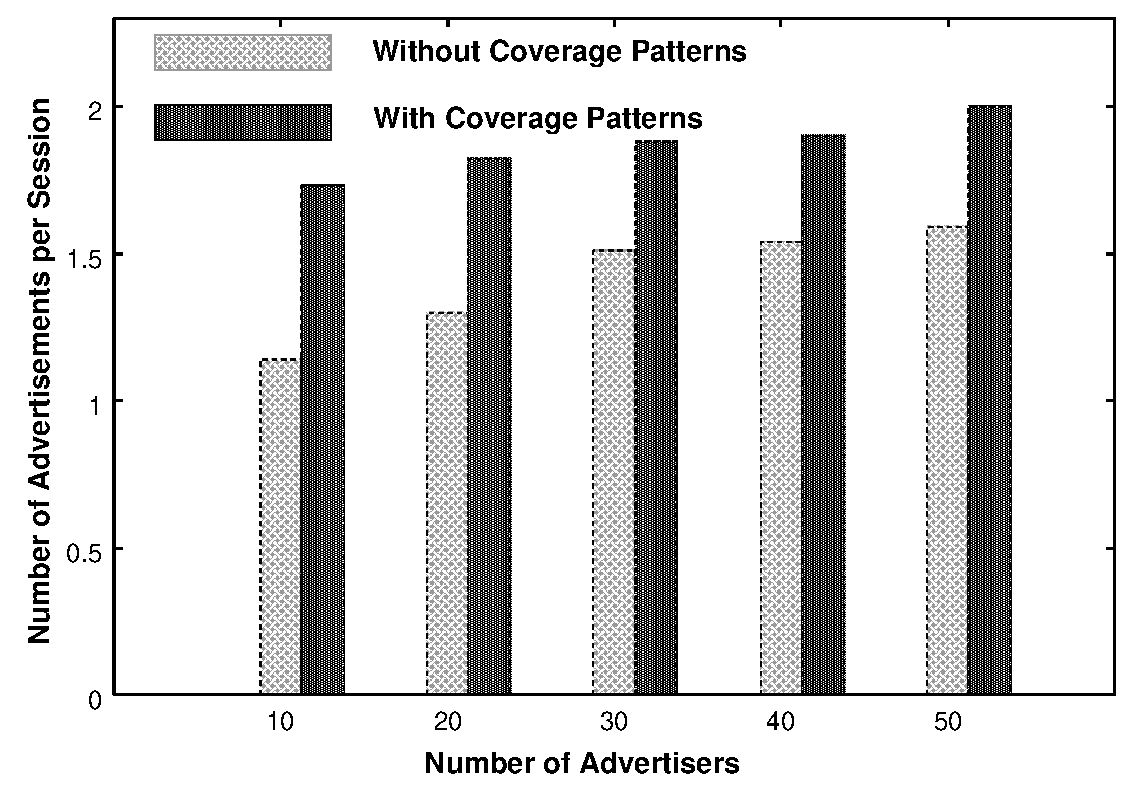
\includegraphics[width=7cm]{Results/shopping_1_obj.eps} }}%
  \qquad
  \subfloat[Category--Society]{{\includegraphics[width=7cm]{Results/society_1_obj.eps} }}%
	\qquad
	 \subfloat[Category--Arts]{{\includegraphics[width=7cm]{Results/arts_1_obj.eps} }}%
 	\qquad
	 \subfloat[Category--health]{{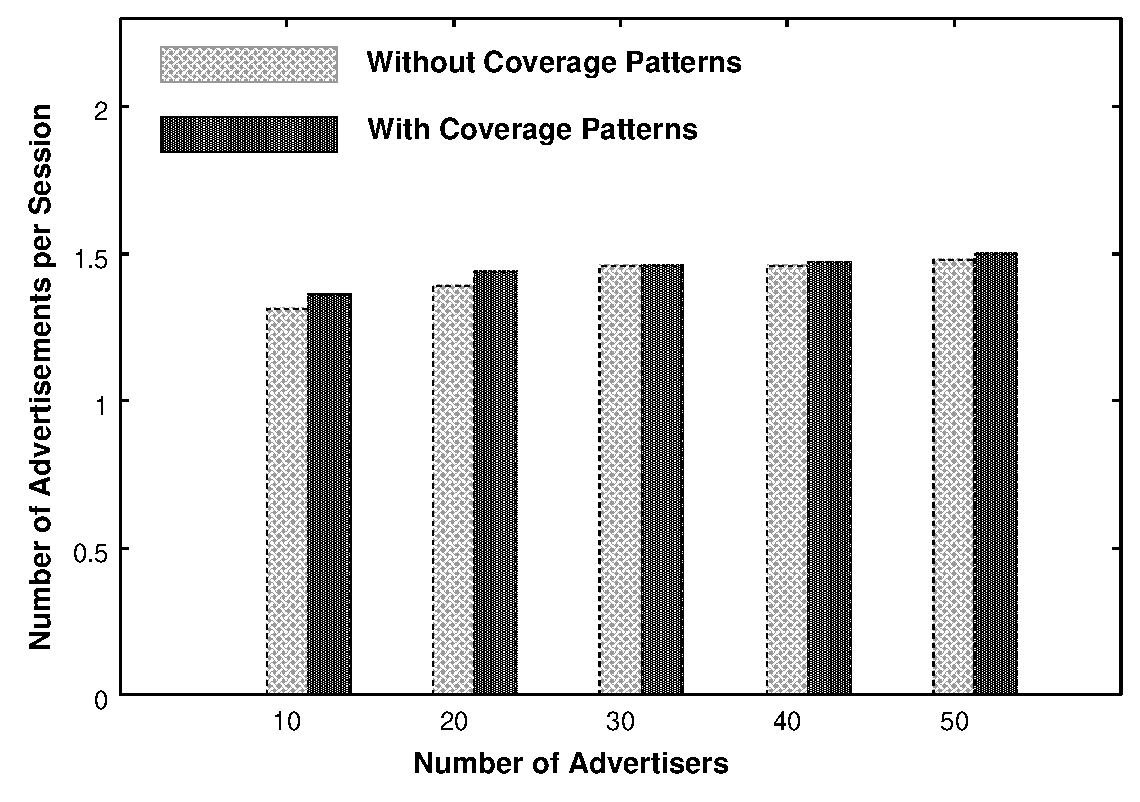
\includegraphics[width=7cm]{Results/health_1_obj.eps} }}%
  \caption{Performance with Respect to Coverage of Advertisers }%
  \label{fig:results-parameter2}%
\end{figure}

Figure \ref{fig:results-parameter2} show a comparison of sponsored search architecture with and without coverage patterns. It can be observed that there is a significant improvement in the performance of AS for each category.  For {\it Shopping, Arts, Society} and {\it Health}, with respect to utilization of sessions, an increase of 33.08\%, 15.81\%, 14\% and 1.89\% was realized with respect to utilization of sessions.  Overall, we observed an increase of 16.20\% in the utilization of sessions.
This is due to the fact that the allocation of advertisements with the proposed approach is able to cover more advertisers by grouping the infrequent keywords. It can be observed that the average session length is 2.5 queries. Even though the session length is small, the experiment results show that the knowledge of  coverage patterns is able to improve the performance. We expect  that in class of applications with large session length, the knowledge of coverage patterns could improve the performance significantly.

It can be also observed that the performance of the proposed approach under all categories is not the same. Especially, for {\it Health} category there is no significant performance improvement. This is due to the fact that the coverage patters extracted for this category have high coverage support and high overlap ratio. Therefore, the number of unique eyeballs is relatively less compared to other categories.



Figure \ref{fig:results:parameter1} shows the performance of two approaches regarding diversity. It can be observed that there is a significant improvement in performance of SA for each category.  In the category of {\it Shopping} an increase of 26.13\% in the diversity was noted while for the categories of {\it Arts}, {\it Society} and {\it Health}, it was 6.62\% , 21.98\% and 14.85\% respectively. On an average, we noticed an increase of 17.39\% in the diversity in the proposed approach. The variation in the diversity performance occurs due to search behavioral patterns pertaining to each category.


\begin{figure}[h]
	
  \centering
  \subfloat[Category--Shopping]{{\includegraphics[width=7cm]{Results/shopping_obj.eps} }}%
  \qquad
  \subfloat[Category--Society]{{\includegraphics[width=7cm]{Results/society_obj.eps} }}%
	\qquad
	 \subfloat[Category--Arts]{{\includegraphics[width=7cm]{Results/arts_obj.eps} }}%
	\qquad
 \subfloat[Category--Health]{{\includegraphics[width=7cm]{Results/health_obj.eps} }}%

  \caption{Performance with respect to Diversity}%
 \label{fig:results:parameter1}%
\end{figure}



\section{Discussion: Assumptions and Limitations}

\label{Ch4Discussion}

The proposed approach has the following assumptions and limitations:

\begin{enumerate}[label=(\roman*).]

\item We have assumed that bidding on concepts is more natural compared to bidding on keywords as concepts communicate integrated ideas which is not the case with individual keywords. Our motivation to bid on concepts also comes from social media advertising where advertisers select demographic concepts like photography, reading, travelling, lifestyle, etc. The approach of bidding on concepts has been quite successful in social media advertising. 

\item It is assumed that the transactions formed from web query logs can be used to identify the set of concepts that cover a given percentage of visitor population. Such knowledge could be used to place the advertisement assuming similar search behavior. The related issues will be
investigated as a part of future work.

\item We have also made the assumption that each query and ad pair within the same high level concept are relevant to each other. Overall, this assumption may be true but more analysis is needed on how to do targeted advertising similar to the approach of bidding on keywords. Moreover, we also assume that if an advertiser is bidding on a high level node in the taxonomy, he/she is interested in showing his/her ad on a query which belongs to any descendant of the bidding node.

\item There is a need to understand the interplay between more relevant queries and increase in reach of audiences. More reach of an ad might also mean that ad is being shown to irrelevant users, thereby compromising the user experience and brand perception.

\item Bidding is only performed on the first level of the taxonomy. This might not be suitable for all the advertisers as the advertising requirements for each advertiser is different.

\end{enumerate}







\section{Summary}
\label{ch4Summary}
In this chapter, we have discussed the first approach for long tail advertising in sponsored search. We proposed that advertisers should bid upon high level concepts instead of individual keywords in ad space auctions. Using session based transactions, we extracted coverage patterns from search query logs and performed a matching between extracted coverage patterns and advertising demands. We further proposed an end-to-end framework to use this matching to allocate ads to incoming search queries. Experimental results on a real world dataset also showed improvement with respect to utilization of ad space and reach of advertisements. 


